
\begin{figure}
    \begin{fullwidth}
    \centering{
        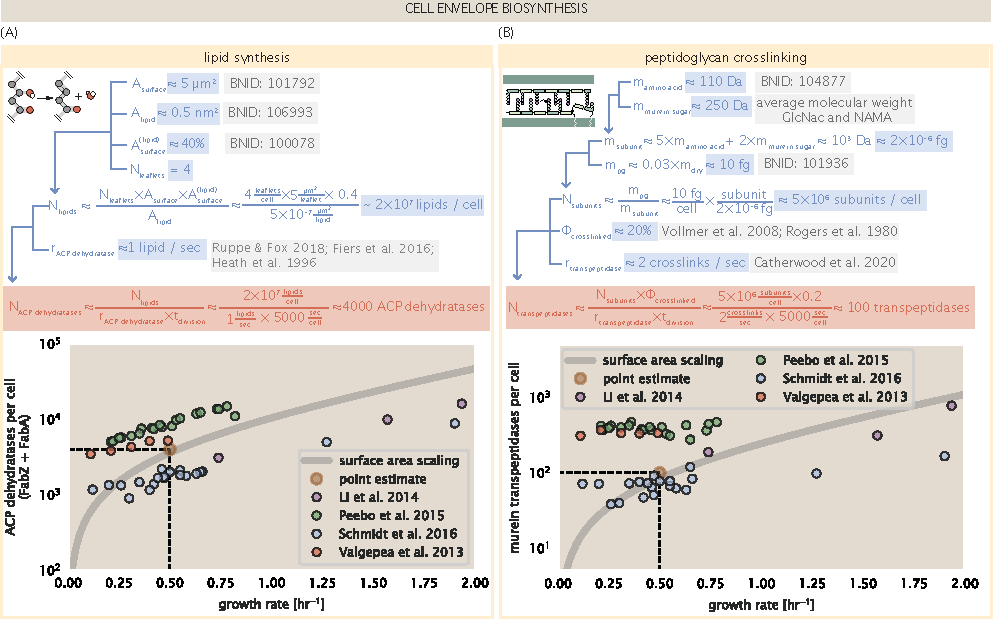
\includegraphics{main_figs/cell_wall_peptidoglycan.pdf}
        \caption{\textbf{Estimation of the key components involved in cell
        envelope biosynthesis.} (A) Top panel shows an estimation for
        the number of ACP dehydratases necessary to form functional
        phospholipids, which is assumed to be a rate-limiting step on lipid synthesis. The rate of ACP dehydratases was inferred from
        experimental measurements via a stochastic kinetic model described in
        \cite{ruppe2018}. Bottom panel shows the experimentally observed complex
        copy numbers using the stoichiometries [FabA]$_2$ and [FabZ]$_2$. (B) An
        estimate for the number of peptidoglycan transpeptidases needed to
        complete maturation of the peptidoglycan. The mass of the murein monomer
        was estimated by approximating each amino acid in the pentapeptide chain
        as having a mass of 110 Da and each sugar in the disaccharide having a
        mass of $\approx$ 250 Da. The \textit{in vivo} rate of transpeptidation
        rein \textit{E. coli} was taken from recent analysis by
        \cite{catherwood2020}. The bottom panel shows experimental measurements
        of the transpeptidase complexes in \textit{E. coli} following the
        stoichiometries [MrcA]$_2$, [MrcB]$_2$, [MrdA]$_1$, and [MrdB]$_1$. Grey
        curves in each plot show the estimated number of complexes needed to
        satisfy the synthesis requirements scaled by the surface area as a
        function of growth rate. We direct the reader to the supplemental
        information for a more detailed discussion of this estimate.
        }
        \label{fig:cell_envelope}
    }
    \end{fullwidth}

\end{figure}
